\documentclass[10pt,a4paper]{article}
\usepackage{amsmath}
\usepackage{amssymb}
\usepackage{graphicx}
\usepackage{color}
\usepackage{fancyhdr}
\usepackage{fancyvrb}
\usepackage[margin=3.5cm]{geometry}
\usepackage{framed}
\usepackage{enumerate}
\usepackage{textcomp}
\def\ket#1{\left|#1\right\rangle}
\def\bra#1{\left\langle#1\right|}
\def\braket#1{\left\langle#1\right\rangle}

\definecolor{linkcol}{rgb}{0.0, 0.0, 0.7}
\usepackage[colorlinks=true,urlcolor=linkcol,citecolor=black,linkcolor=linkcol]{hyperref}

\setcounter{section}{6}
\renewcommand\thesection{\arabic{section}}
\renewcommand\thesubsection{\thesection.\arabic{subsection}}

\fancyhf{}
\lhead{\tiny Y.~D.~Chong (2020)}
\rhead{\scriptsize MH2801: Complex Methods for the Sciences}
\lfoot{}
\rfoot{\thepage}
\pagestyle{fancy}

\begin{document}
\setcounter{page}{50}

\section{Branch Points and Branch Cuts}
\label{branch-points-and-branch-cuts}

When introducing complex algebra, we postponed discussion of what it
means to raise a complex number to a non-integer power, such as
$z^{1/2}$, $z^{4/3}$, or $z^{\pi}$. It is now time to open that
can of worms. This involves learning about the two indispensible
concepts of \textbf{branch points} and \textbf{branch cuts}.

\subsection{Non-integer powers as multi-valued operations}
\label{non-integer-powers-as-multi-valued-operations}

Given a complex number in its polar representation, $z =
r\exp[i\theta]$, raising to the power of $p$ could be handled this
way:
\begin{equation}
z^p = \left(re^{i\theta}\right)^p = r^p e^{ip\theta}.
\end{equation}
Let's take a closer look at the complex exponential term
$e^{ip\theta}$. Since $\theta = \mathrm{arg}(z)$ is an angle, we can
change it by any integer multiple of $2\pi$ without altering the value
of $z$. Taking this fact into account, we can re-write the above
equation more carefully as
\begin{equation}
z^p = \left(r\,e^{i(\theta + 2\pi n)}\right)^p = \left(r^p e^{ip\theta} \right) e^{2\pi i n p} \quad\; \mathrm{where}\;\; n\in\mathbb{Z}.
\end{equation}
Thus, there is an ambiguous factor of $\exp(2\pi i n p)$, where $n$ is
any integer. If $p$ is an integer, there is no problem, since $2\pi n
p$ will be an integer multiple of $2\pi$, so $z^p$ has the same value
regardless of $n$:
\begin{equation}
z^p = r^p e^{ip\theta} \;\;\textrm{unambiguously} \;\;\;(\text{if}\,p\in\mathbb{Z}).
\end{equation}
But if $p$ is not an integer, there is no unique answer, since
$\exp\left(2 \pi i np\right)$ has different values for different
$n$. In that case, ``raising to the power of $p$'' is a
\textbf{multi-valued operation}.  It cannot be treated as a function
in the usual sense, since functions must have unambiguous outputs (see
Chapter 0).

\subsubsection{Roots of unity}\label{roots-of-unity}

Let's take a closer look at the problematic exponential term,
\begin{equation}
\exp\left(2\pi i np\right), \quad n \in \mathbb{Z}.
\end{equation}
If $p$ is irrational, $2\pi np$ never repeats itself modulo $2\pi$.
Thus, $z^p$ has an infinite set of values, one for each integer $n$.

More interesting is the case of a non-integer \emph{rational} power,
which can be written as $p = P/Q$ where $P$ and $Q$ are integers with
no common divisor.  It can be proven using
\href{https://en.wikipedia.org/wiki/Modular_arithmetic}{modular
  arithmetic} (though we will not go into the details) that $2\pi n\,
(P/Q)$ has exactly $Q$ unique values modulo $2\pi$:
\begin{equation}
 2\pi n\, \left(\frac{P}{Q}\right) = 2\pi \times \left\{0,\, \frac{1}{Q},\, \frac{2}{Q},\, \dots, \frac{(Q-1)}{Q} \right\} \quad(\mathrm{modulo} \; 2\pi).
\end{equation}
This set of values is independent of the numerator $P$, which merely
affects the sequence in which the numbers are generated. We can
clarify this using a few simple examples:

\begin{framed} \noindent
\textit{Example}---Consider the complex square root operation,
$z^{1/2}$. If we write $z$ in its polar respresentation,
\begin{equation}
  z = r e^{i\theta},
\end{equation}
then
\begin{equation}
  z^{1/2} = \left[r \, e^{i(\theta + 2 \pi n)} \right]^{1/2} = r^{1/2} \, e^{i\theta/2} \, e^{i \pi n}, \quad n \in \mathbb{Z}.
\end{equation}
The factor of $e^{i\pi n}$ has two possible values: $+1$ for even
$n$, and $-1$ for odd $n$. Hence,
\begin{equation}
  z^{1/2} = r^{1/2} \, e^{i\theta/2} \;\times\; \left\{1, -1\right\}.
\end{equation}
\end{framed}

\begin{framed} \noindent
  \textit{Example}---Consider the cube root operation
  $z^{1/3}$. Again, we write $z$ in its polar representation, and
  obtain
\begin{equation}
z^{1/3} = r^{1/3} \, e^{i\theta/3} \, e^{2\pi i n/3}, \quad n \in \mathbb{Z}.
\end{equation}
The factor of $\exp(2\pi i n/3)$ has the following values for
different $n$:
\begin{equation*}
\begin{array}{|c||c|c|c|c|c|c|c|c|c|} \hline n &\cdots & -2 & -1 & 0 & 1 & 2 & 3 & 4 & \cdots \\ \hline e^{2\pi i n/3} &\cdots & e^{2\pi i /3} & e^{-2\pi i /3} & \;\,\;1\;\,\; & e^{2\pi i /3} & e^{-2\pi i /3} & \;\,\;1\;\,\; & e^{2\pi i /3} & \cdots \\ \hline \end{array}
\end{equation*}
From the pattern, we see that there are three possible values of the
exponential factor:
\begin{equation}
e^{2\pi i n/3} = \left\{1, e^{2\pi i /3}, e^{-2\pi i /3}\right\}.
\end{equation}
Therefore, the cube root operation has three distinct values:
\begin{equation}
z^{1/3} = r^{1/3} \, e^{i\theta/3} \;\times\; \left\{1, e^{2\pi i /3}, e^{-2\pi i /3}\right\}.
\end{equation}
\end{framed}

%% \vskip 0.15in

\begin{framed} \noindent
  \textit{Example}---Consider the operation $z^{2/3}$. Again, writing
  $z$ in its polar representation,
\begin{equation}
z^{2/3} = r^{2/3} \, e^{2i\theta/3} \, e^{4\pi i n/3}, \quad n \in \mathbb{Z}.
\end{equation}
The factor of $\exp(4\pi i n/3)$ has the following values for
different $n$:
\begin{equation*}
\begin{array}{|c||c|c|c|c|c|c|c|c|c|} \hline n &\cdots & -2 & -1 & 0 & 1 & 2 & 3 & 4 & \cdots \\ \hline e^{4\pi i n/3} &\cdots & e^{-2\pi i /3} & e^{2\pi i /3} & \;\,\;1\;\,\; & e^{-2\pi i /3} & e^{2\pi i /3} & \;\,\;1\;\,\; & e^{-2\pi i /3} & \cdots \\ \hline \end{array}
\end{equation*}
Hence, there are three possible values of this exponential factor,
\begin{equation}
e^{2\pi i n (2/3)} = \left\{1, e^{2\pi i /3}, e^{-2\pi i /3}\right\}.
\end{equation}
Note that this is the exact same set we obtained for $e^{2\pi i n/3}$
in the previous example, in agreement with the earlier assertion that
the numerator $P$ has no effect on the set of values.  Thus,
\begin{equation}
z^{2/3} = r^{2/3} \, e^{2i\theta/3} \;\times\; \left\{1, e^{2\pi i /3}, e^{-2\pi i /3}\right\}.
\end{equation}
\end{framed}

%% \vskip 0.2in

From the above examples, we deduce the following expression for
rational powers:
\begin{equation}
z^{P/Q} = r^{P/Q} \; e^{i\theta\, (P/Q)}\, \times \left\{1,\, e^{2\pi i \cdot (1/Q)},\, e^{2\pi i \cdot (2/Q)},\, \dots, e^{2\pi i \cdot [(1-Q)/Q]} \right\}.
\end{equation}
The quantities in the curly brackets are called the \textbf{roots of
  unity}. In the complex plane, they sit at $Q$ evenly-spaced points
on the unit circle, with $1$ as one of the values:

\begin{figure}[ht]
  \centering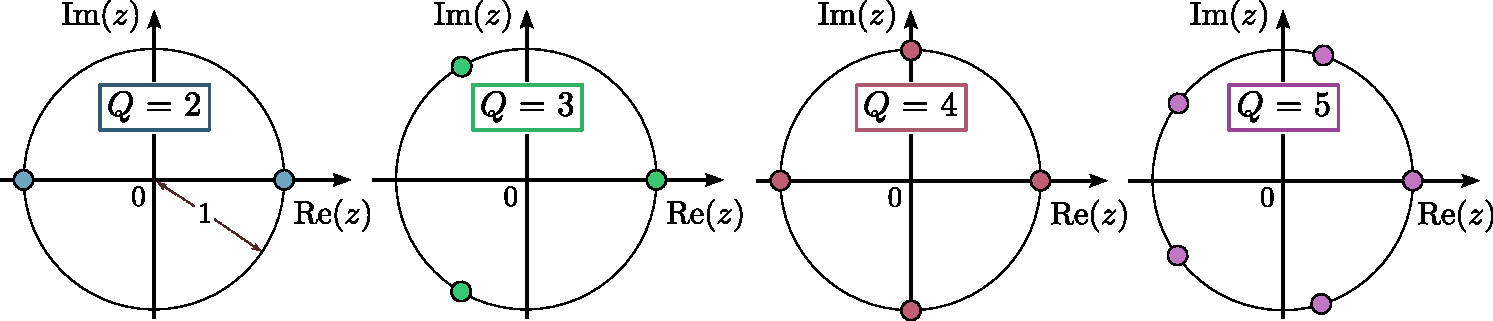
\includegraphics[width=0.95\textwidth]{roots_of_unity}
\end{figure}

\subsubsection{Complex logarithms}\label{complex-logarithms}

Here is another way to think about non-integer powers.  Recall what it
means to raise a number to, say, the power of 5: we simply multiply
the number by itself five times. What about raising a number to a
non-integer power $p$? For the real case, we used the following
definition based on a combination of exponential and logarithm
functions:
\begin{equation}
x^p \equiv \exp\,\left[\,p\ln(x)\right].
\end{equation}
This definition relies on the fact that, for real inputs, the
logarithm is a well-defined function. That, in turn, comes from the
definition of the logarithm as the inverse of the exponential
function. Since the real exponential is one-to-one, its inverse is
also one-to-one.

The complex exponential, however, is many-to-one, since changing its
input by any multiple of $2\pi i$ yields the same output:
\begin{equation}
\exp(z + 2\pi i n) = \exp(z) \cdot e^{2\pi i n} = \exp(z) \quad \forall\; n \in \mathbb{Z}.
\end{equation}
The inverse of the complex exponential is the \textbf{complex
logarithm}. Since the complex exponential is many-to-one, the complex
logarithm does not have a unique output. Instead, $\ln(z)$ refers to
an infinite discrete set of values, separated by integer multiples of
$2\pi i$. We can express this state of affairs in the following way:
\begin{equation}
\ln(z) = \big[\ln(z)\big]_{\mathrm{p.v.}}\; +\; 2 \pi i n, \quad n \in \mathbb{Z}.
\label{logformula}
\end{equation}
Here, $[\ln(z)]_{\mathrm{p.v.}}$ denotes the \textbf{principal value}
of $\ln(z)$, which refers to a reference value of the logarithm
operation (which we'll define later).  Do not think of the principal
value as the "actual" result of the $\ln(z)$ operation! There are
multiple values, each equally legitimate; the principal value is
merely one of these possible results.

Plugging Eq.~\eqref{logformula} into the formula $z^p \equiv
\exp\left[p\ln(z)\right]$ gives
\begin{align}
  z^p &= \exp\Big\{p\big([\ln(z)]_{\mathrm{p.v.}} + 2\pi i n\big)\Big\}\\
  &= \exp\Big\{p[\ln(z)]_{\mathrm{p.v.}}\Big\} \times e^{2\pi i np}, \quad n \in \mathbb{Z}.
\end{align}
The final factor, which is responsible for the multi-valuedness, are
the roots of unity found in Section \ref{roots-of-unity}.

\subsection{Branches}\label{branches}

We have discussed two examples of multi-valued complex operations:
non-integer powers and the complex logarithm.  However, we usually
prefer to deal with functions rather than multi-valued operations. One
major motivating factor is that the concept of the complex derivative
was formulated in terms of functions, not multi-valued operations.

There is a standard procedure to convert multi-valued operations into
functions. First, we define one or more curve(s) in the complex plane,
called \textbf{branch cuts} (the reason for this name will be
explained later). Next, we modify the domain (i.e., the set of
permissible inputs) by excluding all values of $z$ lying on a branch
cut. Then the outputs of the multi-valued operation can be grouped
into discrete \textbf{branches}, with each branch behaving just like a
function.

The above procedure can be understood through the example of the
square root.

\subsubsection{Branches of the complex square root}
\label{branches-of-the-complex-square-root}

As we saw in Section~\ref{roots-of-unity}, the complex square root,
$z^{1/2}$, has two possible values.  We can define the two branches as
follows:

\begin{enumerate}
\item 
Define a branch cut along the negative real axis, so that the domain
excludes all values of $z$ along the branch cut. In in other words, we
will only consider complex numbers whose polar representation can be
written as
\begin{equation}
z = r e^{i\theta}, \quad \theta \in (-\pi, \pi).
\end{equation}
(For those unfamiliar with this notation, $\theta \in (-\pi, \pi)$
refers to the interval $-\pi < \theta < \pi$. The parentheses indicate
that the boundary values of $-\pi$ and $\pi$ are excluded. By
contrast, we would write $\theta \in [-\pi, \pi]$ to refer to the
interval $-\pi \le \theta \le \pi$, with the square brackets
indicating that the boundary values are included.)

\item
  One branch is associated with the $+1$ root. On this branch, for $z
  = re^{i\theta}$, the value is
  \begin{equation}
    f_+(z) = r^{1/2} \, e^{i\theta/2}, \quad \theta \in (-\pi, \pi).
  \end{equation}

\item
  The other branch is associated with the root of unity $-1$. On this
  branch, the value is
\begin{equation}
f_-(z) = -r^{1/2} \, e^{i\theta/2}, \quad \theta \in (-\pi, \pi).
\end{equation}
\end{enumerate}

\noindent
In the following plot, you can observe how varying $z$ affects the
positions of $f_+(z)$ and $f_-(z)$ in the complex plane:

\begin{figure}[h]
  \centering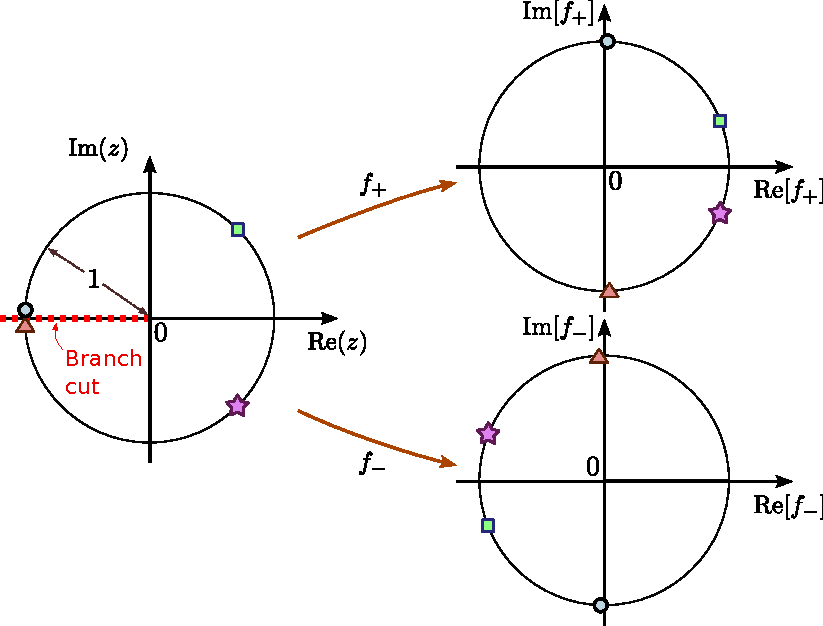
\includegraphics[width=0.75\textwidth]{complex_root_1}
\end{figure}

The red dashed line in the left plot indicates the branch cut. Our
definitions of $f_+(z)$ and $f_-(z)$ implicitly depend on the choice
to place the branch cut on the negative real axis, which led to the
representation of the argument of $z$ as $\theta \in (-\pi,\pi)$.

In the above figure, note that $f_+(z)$ always lies in the right half
of the complex plane, whereas $f_-(z)$ lies in the left half of the
complex plane.  Both $f_+$ and $f_-$ are well-defined functions with
unambiguous outputs, albeit with domains that do not cover the entire
complex plane.  Moreover, they are analytic over their entire domain
(i.e., all of the complex plane except the branch cut); this can be
proven using the Cauchy-Riemann equations, and is left as an exercise.

The end-point of the branch cut is called a \textbf{branch point}.
For $z = 0$, both branches give the same result: $f_+(0) = f_-(0) =
0$. We will have more to say about branch points in Section
\ref{branch-points}.

\subsubsection{Different branch cuts for the complex square root}
\label{different-branch-cuts-for-the-complex-square-root}

In the above example, you may be wondering why the branch cut has to
lie along the negative real axis. In fact, this choice is not
unique. For instance, we could place the branch cut along the positive
real axis. This corresponds to specifying the input $z$ using a
different interval for $\theta$:
\begin{equation}
z = re^{i\theta}, \quad \theta \in (0, 2\pi).
\end{equation}
Next, we use the same formulas as before to define the branches of the
complex square root:
\begin{equation}
f_\pm(z) = \pm r^{1/2} \, e^{i\theta/2}.
\end{equation}
But because the domain of $\theta$ has been changed to $(0, 2\pi)$,
the set of inputs $z$ now excludes the positive real axis. With this
new choice of branch cut, the branches are shown in the following
figure.

\begin{figure}[h]
  \centering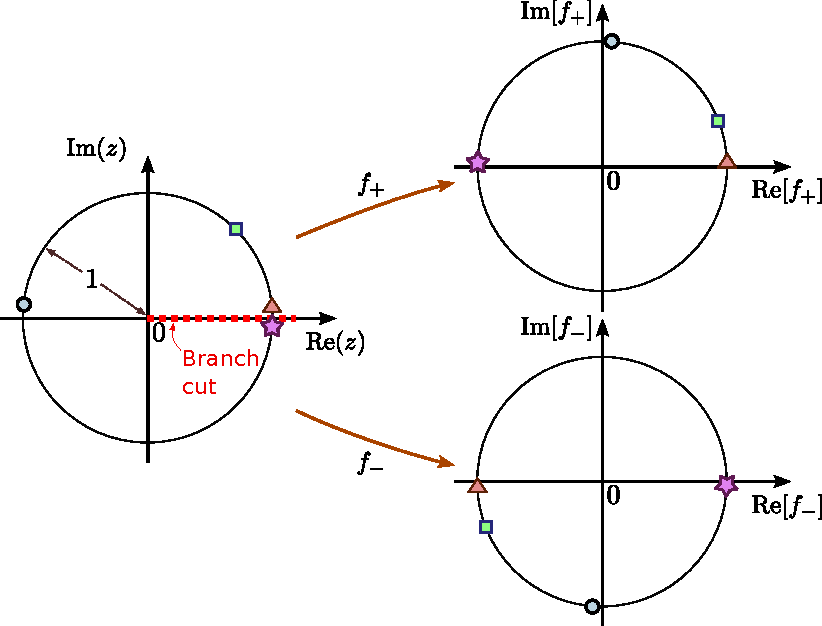
\includegraphics[width=0.75\textwidth]{complex_root_2}
\end{figure}

These two branch functions are different from what we had before. Now,
$f_+(z)$ is always in the upper half of the complex plane, and
$f_-(z)$ in the lower half of the complex plane. However, both
branches still have the same value at the branch point: $f_+(0) =
f_-(0) = 0$.

The branch cut serves as a boundary where two branches are ``glued''
together. You can think of ``crossing'' a branch cut as having the
effect of moving continuously from one branch to another. In the above
figure, consider the case where $z$ is just above the branch cut. Then
$f_+(z)$ lies just above the positive real axis, and $f_-(z)$ lies
just below the negative real axis. Next, consider $z$ lying just below
the branch cut. This is equivalent to a small downwards displacement
of $z$, ``crossing'' the branch cut. For this case, $f_-(z)$ now lies
just below the positive real axis, near where $f_+(z)$ was
previously. Moreover, $f_+(z)$ now lies just above the negative real
axis, near where $f_-(z)$ was previously. Crossing the branch cut thus
swaps the values of the positive and negative branches.

The three-dimensional plot below provides another way to visualize the
role of the branch cut.  Here,the horizontal axes correspond to
$\mathrm{Re}(z)$ and $\mathrm{Im}(z)$. The vertical axis shows the
arguments for the two values of the complex square root, with
$\mathrm{arg}\big[f_+(z)\big]$ plotted in orange and
$\mathrm{arg}\big[f_-(z)\big]$ plotted in blue. If we vary the choice
of the branch cut, that simply affects which values of the
multi-valued operation are assigned to the $+$ (orange) branch, and
which values are assigned to the $-$ (blue) branch. Hence, the choice
of branch cut is just a choice about how to divide up the branches of
a multi-valued operation.

\begin{figure}[h]
  \centering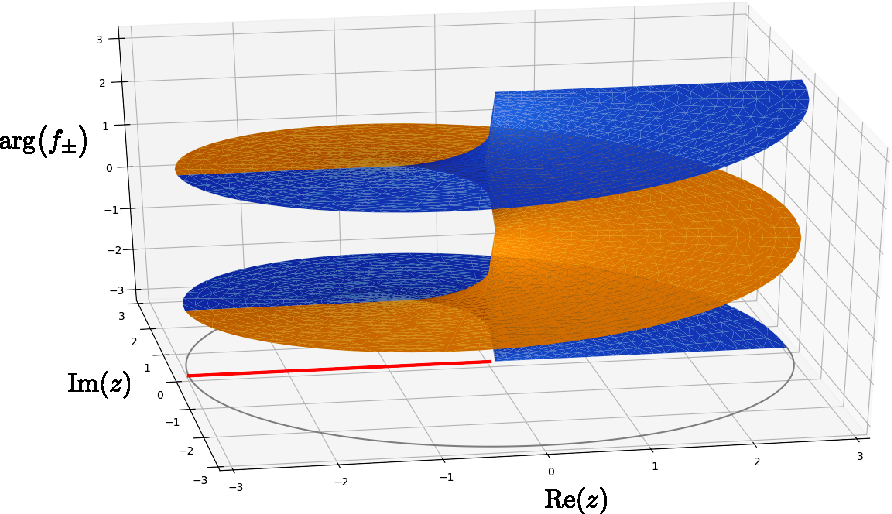
\includegraphics[width=0.7\textwidth]{branches}
\end{figure}

\subsubsection{Branch points}
\label{branch-points}

The tip of each branch cut is called a \textbf{branch point}. A branch
point is a point where the multi-valued operation gives an unambiguous
answer, with different branches giving the same output. Whereas the
choice of branch cuts is non-unique, the positions of the branch points
of a multi-valued operation are uniquely determined.

For the purposes of this course, you mostly only need to remember the
branch points for two common cases:

\begin{itemize}
\item
  The $z^p$ operation (for non-integer $p$) has branch points at $z =
  0$ and $z = \infty$. For rational powers $p = P/Q$, where $P$ and
  $Q$ have no common divisor, there are $Q$ branches, one for each
  root of unity. At each branch point, all $Q$ branches meet.
\item
  The complex logarithm has branch points at $z = 0$ and $z =
  \infty$. There is an infinite series of branches, separated from
  each other by multiples of $2 \pi i$. At each branch point, all the
  branches meet.
\end{itemize}

\noindent
We can easily see that $z^p$ must have a branch point at $z = 0$: its
only possible value at the origin is $0$, regardless of which root of
unity we choose. To understand the other branch points listed above, a
clearer understanding of the concept of ``infinity'' for complex
numbers is required, so we will discuss that now.

\subsection{Aside: the meaning of ``infinity'' for complex numbers}
\label{aside-the-meaning-of-infinity-for-complex-numbers}

When talking about $z = \infty$, we are referring to something called
\textbf{complex infinity}, which can be regarded as a complex number
with infinite magnitude and \emph{undefined} argument.

The fact that the argument is undefined may seem strange, but actually
we already know of another complex number with this feature: $z = 0$
has zero magnitude and undefined argument.  These two special complex
numbers are the reciprocals of each other: $1/\infty = 0$ and $1/0 =
\infty$.

The complex $\infty$ behaves differently from the familiar concept of
infinity associated with real numbers. For real numbers, positive
infinity ($+\infty$) is distinct from negative infinity
($-\infty$). But this doesn't hold for complex numbers, since complex
numbers occupy a two-dimensional plane rather than a line. Thus, for
complex numbers it does not make sense to define ``positive infinity''
and ``negative infinity'' as distinct entities. Instead, we work with
a single complex $\infty$.

From this discussion, we can see why $z^p$ is has a branch point at $z
= \infty$. For any finite and nonzero $z$, we can write $z =
re^{i\theta}$, where $r$ is a positive number. The $z^p$ operation
then yields a set of complex numbers of the form $r^p \,
e^{ip\theta}\,\times\, \{\text{root of unity}\}$.  For each number in
this set, the magnitude goes to infinity as $r \rightarrow \infty$. In
this limit, the argument (i.e., the choice of root of unity) becomes
irrelevant, and the result is simply $\infty$.

By similar reasoning, one can prove that $\ln(z)$ has branch points at
$z = 0$ and $z = \infty$.  This is left as an exercise.

\subsection{Branch cuts for general multi-valued operations}
\label{branch-cuts-for-general-multi-valued-operations}

Having discussed the simplest multi-valued operations, $z^p$ and
$\ln(z)$, here is how to assign branch cuts for more general
multi-valued operations. This is a two-step process:

\begin{enumerate}
\item
Locate the branch points.

\item Assign branch cuts in the complex plane, such that:
  \begin{itemize}
  \item Every branch point has a branch cut ending on it.
  \item Every branch cut ends on a branch point.
  \end{itemize}
  Note that any branch point lying at infinity must also obey these
  rules.  The branch cuts should not intersect.
\end{enumerate}

\noindent
The choice of where to place branch cuts is not unique. Branch cuts are
usually chosen to be straight lines, for simplicity, but this is not
necessary. Different choices of branch cuts correspond to different ways
of partitioning the values of the multi-valued operation into separate
branches.

\subsubsection{An important example}
\label{an-important-example}

We can illustrate the process of assigning branch cuts, and defining
branch functions, using the following nontrivial multi-valued
operation:
\begin{equation}
f(z) = \ln\left(\frac{z+1}{z-1}\right).
\end{equation}
This is multi-valued because of the presence of the complex
logarithm. The branch points are $z = 1$ and $z = -1$, as these are
the points where the input to the logarithm becomes $\infty$ or $0$
respectively. Note that $z = \infty$ is *not* a branch point; at $z =
\infty$, the input to the logarithm is $-1$, which is not a branch
point for the logarithm.

We can assign any branch cut that joins these two. A convenient choice
is shown below:

\begin{center}
  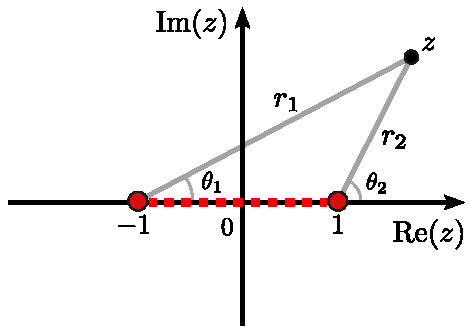
\includegraphics[width=0.4\textwidth]{branch_cut_example}
\end{center}

\noindent
This choice of branch cut is nice because we can express the $z+1$ and
$z - 1$ terms using the polar representations
\begin{align}
  z + 1 &= r_1\,e^{i\theta_1}, \\
  z - 1 &= r_2\, e^{i\theta_2},
\end{align}
where $r_1$, $r_2$, $\theta_1$, and $\theta_2$ are shown
graphically in the above figure. The positioning of the branch cut
corresponds to a particular choice for the ranges of the complex
arguments $\theta_1$ and $\theta_2$. As we'll shortly see, the
present choice of branch cut corresponds to
\begin{equation}
\theta_1 \in (-\pi,\pi), \quad \theta_2 \in (-\pi,\pi).
\end{equation}
Hence, in terms of this polar representation, $f(z)$ can be written as
\begin{align}
  \begin{aligned}
    f(z) = \ln\left(\frac{r_1}{r_2}\right) + i(\theta_1 - \theta_2 + 2\pi m), \quad m\in\mathbb{Z}, \\
    \mathrm{where}\; z = -1 + r_1\,e^{i\theta_1} = 1 + r_2\,e^{i\theta_2},\quad\theta_1, \theta_2 \in (-\pi,\pi).
  \end{aligned}
\end{align}
The choice of $m$ specifies the branch, and we can choose $m = 0$ as
the principal branch.

Let's now verify that setting $\theta_1 \in (-\pi,\pi)$ and
$\theta_2 \in (-\pi,\pi)$ is consistent with our choice of branch cut.
Consider the principal branch, and compare the outputs of the above
formula for $z$ just above the real axis, and for $z$ just below the
real axis. There are three cases of interest. Firstly, for
$\mathrm{Re}(z) < 1$ (to the left of the leftmost branch point),
\begin{align}
  \mathrm{Im}(z) &= 0^+ \;\;\Rightarrow\;\; f(z) = \ln\left(\frac{r_1}{r_2}\right) + i\Big((\pi) - (\pi)\Big) \quad = \ln\left(\frac{r_1}{r_2}\right) \\ \mathrm{Im}(z) &= 0^- \;\;\Rightarrow \;\; f(z) = \ln\left(\frac{r_1}{r_2}\right) + i\Big((-\pi) - (-\pi)\Big) = \ln\left(\frac{r_1}{r_2}\right).
\end{align}
Thus, there is no discontinuity along this segment of the real axis.

Secondly, for $-1 < \mathrm{Re}(z) < 1$ (between the two branch
points),
\begin{align}
  \mathrm{Im}(z) &= 0^+ \;\;\Rightarrow\;\; f(z) = \ln\left(\frac{r_1}{r_2}\right) + i\Big((0) - (\pi)\Big) \;\;= \ln\left(\frac{r_1}{r_2}\right) -i\pi \\ \mathrm{Im}(z) &= 0^- \;\;\Rightarrow\;\; f(z) = \ln\left(\frac{r_1}{r_2}\right) + i\Big((0) - (-\pi)\Big) = \ln\left(\frac{r_1}{r_2}\right) + i\pi.
\end{align}
Hence, in the segment between the two branch points, there is a
discontinuity of $\pm 2\pi i$ on different sides of the real axis. The
value of this discontinuity is exactly equal, of course, to the
separation between the different branches of the complex logarithm.

Finally, for $\mathrm{Re}(z) > 1$ (to the right of the rightmost
branch point), there is again no discontinuity:
\begin{align}
  \mathrm{Im}(z) &= 0^+ \;\;\Rightarrow\;\; f(z) = \ln\left(\frac{r_1}{r_2}\right) + i\Big((0) - (0)\Big) = \ln\left(\frac{r_1}{r_2}\right) \\ \mathrm{Im}(z) &= 0^- \;\;\Rightarrow\;\; f(z) = \ln\left(\frac{r_1}{r_2}\right) + i\Big((0) - (0)\Big) = \ln\left(\frac{r_1}{r_2}\right).
\end{align}

\subsection{Exercises}\label{exercises}

\begin{enumerate}
\item
Find the values of $(i)^i$.

\item
Prove that $\ln(z)$ has branch points at $z = 0$ and $z = \infty$.

\item For each of the following multi-valued functions, find all the possible
function values, at the specified $z$:
\begin{enumerate}
\item $z^{1/3}$ at $z = 1$.

\item $z^{3/5}$ at $z = i$.

\item $\ln(z+i)$ at $z = 1$.

\item $\cos^{-1}(z)$ at $z = i$
\end{enumerate}

\item
For the square root operation $z^{1/2}$, choose a branch cut. Then
show that both the branch functions $f_\pm(z)$ are analytic over all
of $\mathbb{C}$ excluding the branch cut.

\item
  Consider $f(z) = \ln(z+a) - \ln(z-a)$. For simplicity, let $a$ be a
  positive real number. As discussed in
  Section~\ref{an-important-example}, we can write this as
\begin{equation}
f(z) = \ln\left|\frac{z+a}{z-a}\right| + i(\theta_+ - \theta_-), \qquad \theta_\pm \equiv \mathrm{arg}(z\pm a).
\end{equation}
Suppose we represent the arguments as $\theta_+ \in (-\pi,\pi)$ and
$\theta_- \in (-\pi,\pi)$. Explain why this implies a branch cut
consisting of a straight line joining $a$ with $-a$. Using this
representation, calculate the change in $f(z)$ over an infinitesimal
loop encircling $z = a$ or $z = -a$. Calculate also the change in
$f(z)$ over a loop of radius $R \gg a$ encircling the origin (and
thus enclosing both branch points).
\end{enumerate}
\end{document}
